%%%%%%%%%%%%%%%%%%%%%%%%%%%%%%%%%%%%%%%%%%%%%%%%%%%%%%%%%%%%%%%%%%%%%%%%%%%%%%%
% PREAMBOLO COMUNE PER APPUNTI (Stile Scuro)
%
% Questo file contiene tutte le impostazioni e i pacchetti comuni.
% NON contiene \begin{document} o \end{document}.
%
% Istruzioni per la compilazione del file principale:
% pdflatex -shell-escape nomefile_principale.tex
%%%%%%%%%%%%%%%%%%%%%%%%%%%%%%%%%%%%%%%%%%%%%%%%%%%%%%%%%%%%%%%%%%%%%%%%%%%%%%%

\documentclass{article}

% --- Encoding e lingua ---
\usepackage[utf8]{inputenc}
\usepackage[italian]{babel}

% --- Margini e layout ---
\usepackage{geometry}
\geometry{a4paper, margin=1in}

% --- Font sans-serif (come Helvetica) ---
\usepackage[scaled]{helvet}
\renewcommand{\familydefault}{\sfdefault}
\usepackage[T1]{fontenc}

% --- Matematica ---
\usepackage{amsmath}
\usepackage{amssymb}

% --- Liste personalizzate ---
\usepackage{enumitem}
% \setlist{nosep}

% --- Immagini e Grafica ---
\usepackage{float}
% \usepackage{graphicx}
\usepackage{tikz}
\usetikzlibrary{shapes.geometric, positioning, arrows.meta, calc, fit, backgrounds, patterns, decorations.pathreplacing}

% --- Tabelle Avanzate ---
\usepackage{array}
\usepackage{booktabs}
\usepackage{longtable}

% --- Hyperlink e Metadati PDF ---
\usepackage{hyperref}

\hypersetup{
    colorlinks=true,
    linkcolor=white,
    filecolor=magenta,
    urlcolor=cyan,
    citecolor=green,
    % pdftitle, pdfauthor, ecc. verranno impostati nel file principale
    pdfpagemode=FullScreen,
    bookmarksopen=true,
    bookmarksnumbered=true
}

% --- Licenza del documento ---
\usepackage[
  type={CC},
  modifier={by-sa},
  version={4.0},
]{doclicense}

% --- Colori e Sfondo Nero ---
\usepackage{xcolor}
\pagecolor{black}
\color{white}

% --- Evidenziazione del Codice ---
\usepackage{minted}
\setminted{
    frame=lines,
    framesep=2mm,
    fontsize=\small,
    breaklines=true,
    style=monokai,
    bgcolor=black!80
}
\usemintedstyle{monokai}

% --- Comandi personalizzati per algebra relazionale ---
\newcommand{\Rel}[1]{\textit{#1}} % Per i nomi delle relazioni
\newcommand{\Attr}[1]{\textsf{#1}} % Per i nomi degli attributi

\newcommand{\myunion}{\cup}
\newcommand{\myintersection}{\cap}
\newcommand{\mydifference}{-}
\newcommand{\myrename}[2]{\rho_{#1}(#2)}
\newcommand{\myselectop}[2]{\sigma_{#1}(#2)}
\newcommand{\myproject}[2]{\pi_{#1}(#2)}
\newcommand{\mycartesian}{\times}
\newcommand{\mynaturaljoin}{\bowtie} % Usare \Join da amssymb se disponibile e preferito
\newcommand{\mythetajoin}[3]{#1 \bowtie_{#2} #3} % R1 \bowtie_cond R2

% --- Comandi personalizzati per logica ---
\newcommand{\mylandop}{\wedge}
\newcommand{\myvel}{\vee}
\newcommand{\mynegop}{\neg}
\newcommand{\myforallop}{\forall}
\newcommand{\myexistsop}{\exists}

% --- Join esterni (outer join) ---
% Definizione standard per i join esterni
\def\ojoin{\setbox0=\hbox{$\mynaturaljoin$}%
	\rule[-.02ex]{.25em}{.4pt}\llap{\rule[\ht0]{.25em}{.4pt}}}
\newcommand{\myleftouterjoin}{\mathbin{\ojoin\mkern-5.8mu\mynaturaljoin}}
\newcommand{\myrightouterjoin}{\mathbin{\mynaturaljoin\mkern-5.8mu\ojoin}}
\newcommand{\myfullouterjoin}{\mathbin{\ojoin\mkern-5.8mu\mynaturaljoin\mkern-5.8mu\ojoin}}



\title{Spettro Fisico, Canali Logici, Modulazione Digitale}
\author{Basato sulle slide del Prof. Luciano Bononi}
\date{\today}

\usetikzlibrary{decorations.pathmorphing}

\begin{document}

\maketitle
\tableofcontents
\newpage

\section{Spettro delle Reti Wireless e Allocazione}

\begin{itemize}
    \item \textbf{Spettro Elettromagnetico:} Le comunicazioni wireless utilizzano una porzione dello spettro elettromagnetico, principalmente le \textbf{radiofrequenze}. Questo spettro va da frequenze molto basse (udibili) a frequenze altissime (raggi Gamma).
    \item \textbf{Allocazione delle Frequenze:} Diverse tecnologie wireless operano su diverse bande di frequenza, che sono regolamentate e assegnate per evitare interferenze.
    \begin{itemize}
        \item \textbf{GSM (900/1800 MHz):} Usato per la telefonia mobile 2G.
        \item \textbf{Bluetooth, ZigBee, Wi-Fi (802.11b/g/n) a 2.4 GHz:} Questa è una banda \textbf{ISM (Industrial, Scientific, Medical)}, che è \textit{unlicensed} (non licenziata), il che significa che può essere usata liberamente da dispositivi a bassa potenza, ma è anche più soggetta a interferenze.
        \item \textbf{Wi-Fi (802.11a/ac) a 5 GHz:} Un'altra banda per Wi-Fi, spesso meno affollata della 2.4 GHz.
        \item \textbf{LMDS (Local Multipoint Distribution Service) a 28 GHz:} Usato per accessi wireless a banda larga "ultimo miglio".
        \item \textbf{IR (Infrarosso):} Usato per comunicazioni a cortissimo raggio, come i telecomandi (es. IEEE 802.11 IR).
    \end{itemize}
    \item \textbf{Fixed Spectrum Assignment:} Esiste una mappa globale (anche se con variazioni regionali) che assegna specifiche porzioni di spettro a specifici servizi (es. mobile, broadcasting, aeronautico, ecc.). Questo è fondamentale per l'organizzazione delle comunicazioni.
\end{itemize}
\textit{[Figura di riferimento: Slide 2 - Wireless networks' spectrum, Slide 3 - Fixed spectrum assignment]}

\section{Larghezza di Banda (Bandwidth) e Spettro nelle Reti Wireless}

\begin{itemize}
    \item \textbf{Come i canali wireless possono avere diversa larghezza di banda?}
    \begin{itemize}
        \item \textbf{I bit viaggiano più o meno velocemente? NO.} La velocità di propagazione è vicina a quella della luce (circa $300.000 \text{ Km/s}$) per tutti i bit.
        \item \textbf{Il "tubo" del canale (spettro) è più grande? SÌ/NO.} Avere una porzione di spettro più ampia permette di trasmettere più informazione contemporaneamente.
        \item \textbf{Il canale richiede meno tempo per accomodare (codificare) un bit sul canale? SÌ.} Tecniche di codifica più efficienti permettono di "impacchettare" più bit nello stesso intervallo di tempo o sulla stessa porzione di spettro.
    \end{itemize}
    \item \textbf{Esempio Pratico:}
    Immagina due autostrade: Canale A (1 corsia, 10 auto/ora) e Canale B (2 corsie, 20 auto/ora). Il Canale B ha una "capacità" maggiore. Nelle reti, questo si traduce in più bit/secondo.
\end{itemize}

\begin{figure}[H]
\centering
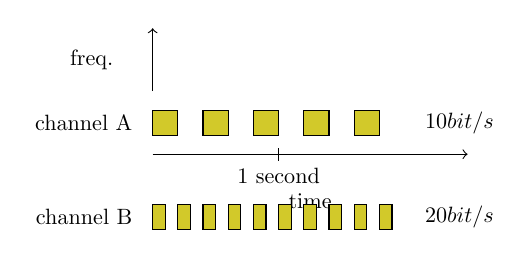
\begin{tikzpicture}[scale=0.8, transform shape]
    % Channel A
    \node[anchor=east] at (-0.5, 2) {freq.};
    \draw[->] (0,1.5) -- (0,2.5);
    \node[anchor=north] at (2.5, 0) {time};
    \draw[->] (0,0.5) -- (5,0.5);
    \node[anchor=east] at (-0.2, 1) {channel A};
    \foreach \i in {0,1,...,4} {
        \fill[yellow!80!black] (\i*0.8, 0.8) rectangle (\i*0.8+0.4, 1.2);
        \draw (\i*0.8, 0.8) rectangle (\i*0.8+0.4, 1.2);
    }
    \node[anchor=west] at (4.2, 1) {$10 \text{ bit/s}$};

    % Channel B
    \node[anchor=east] at (-0.2, -0.5) {channel B};
     \foreach \i in {0,1,...,9} {
        \fill[yellow!80!black] (\i*0.4, -0.7) rectangle (\i*0.4+0.2, -0.3);
        \draw (\i*0.4, -0.7) rectangle (\i*0.4+0.2, -0.3);
    }
    \node[anchor=west] at (4.2, -0.5) {$20 \text{ bit/s}$};
    \draw (2, 0.4) -- (2, 0.6);
    \node[anchor=north] at (2,0.4) {1 second};
\end{tikzpicture}
\caption{Confronto larghezza di banda Canale A vs Canale B.}
\label{fig:bandwidth_comparison}
\end{figure}
\textit{Nell'immagine, il Canale B trasmette il doppio dei bit del Canale A nello stesso secondo.}

\section{Copertura della Trasmissione Radio}
La copertura dipende dalla potenza di trasmissione (Tx power) e dalla sensibilità del ricevitore.

\begin{figure}[H]
\centering
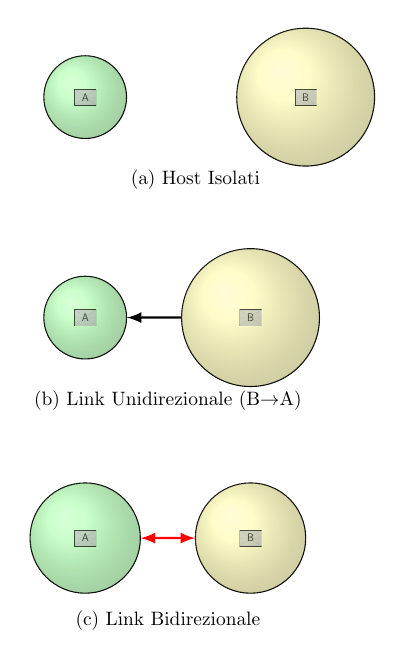
\begin{tikzpicture}[scale=0.7, transform shape]
    % Host Isolati
    \node (A1) [circle, draw, fill=green!20, minimum size=1.5cm, label=center:A] at (0,0) {};
    \node (PC_A1) [scale=0.5] at (A1.center) {\includegraphics[width=0.8cm]{example-image-a}}; % Placeholder for laptop icon
    \shade[ball color=green!30, opacity=0.3] (A1.center) circle (0.75cm);

    \node (B1) [circle, draw, fill=yellow!20, minimum size=2.5cm, label=center:B] at (4,0) {};
    \node (PC_B1) [scale=0.5] at (B1.center) {\includegraphics[width=0.8cm]{example-image-b}}; % Placeholder for laptop icon
    \shade[ball color=yellow!30, opacity=0.3] (B1.center) circle (1.25cm);
    \node at (2,-1.5) {(a) Host Isolati};

    % Link Unidirezionale
    \node (A2) [circle, draw, fill=green!20, minimum size=1.5cm, label=center:A] at (0,-4) {};
    \node (PC_A2) [scale=0.5] at (A2.center) {\includegraphics[width=0.8cm]{example-image-a}};
    \shade[ball color=green!30, opacity=0.3] (A2.center) circle (0.75cm);

    \node (B2) [circle, draw, fill=yellow!20, minimum size=2.5cm, label=center:B] at (3,-4) {};
    \node (PC_B2) [scale=0.5] at (B2.center) {\includegraphics[width=0.8cm]{example-image-b}};
    \shade[ball color=yellow!30, opacity=0.3] (B2.center) circle (1.25cm);
    \draw[-latex, thick] (B2) -- (A2);
    \node at (1.5,-5.5) {(b) Link Unidirezionale (B$\rightarrow$A)};

    % Link Bidirezionale
    \node (A3) [circle, draw, fill=green!20, minimum size=2cm, label=center:A] at (0,-8) {};
    \node (PC_A3) [scale=0.5] at (A3.center) {\includegraphics[width=0.8cm]{example-image-a}};
    \shade[ball color=green!30, opacity=0.3] (A3.center) circle (1cm);

    \node (B3) [circle, draw, fill=yellow!20, minimum size=2cm, label=center:B] at (3,-8) {};
    \node (PC_B3) [scale=0.5] at (B3.center) {\includegraphics[width=0.8cm]{example-image-b}};
    \shade[ball color=yellow!30, opacity=0.3] (B3.center) circle (1cm);
    \draw[latex-latex, thick, red] (A3) -- (B3);
    \node at (1.5,-9.   5) {(c) Link Bidirezionale};
\end{tikzpicture}
\caption{Scenari di copertura radio. (Le icone PC sono placeholder)}
\label{fig:coverage_scenarios}
\end{figure}

\begin{itemize}
    \item \textbf{Host Isolati:} Se due dispositivi (Host A e Host B) hanno una potenza di trasmissione troppo bassa perché i loro segnali si raggiungano, sono isolati (Fig. \ref{fig:coverage_scenarios}a).
    \item \textbf{Link Unidirezionale:} Se Host B ha alta potenza e Host A bassa potenza, A potrebbe ricevere da B, ma B non riceve da A. Questo è un link unidirezionale (talvolta impropriamente detto "asimmetrico" in questo contesto) (Fig. \ref{fig:coverage_scenarios}b).
    \item \textbf{Link Bidirezionale:} Se entrambi hanno potenza sufficiente per raggiungersi a vicenda (Fig. \ref{fig:coverage_scenarios}c).
    \begin{itemize}
        \item \textbf{Link Bidirezionale Simmetrico:} La velocità di trasmissione è la stessa in entrambe le direzioni (es. A$\rightarrow$B 10Mbps, B$\rightarrow$A 10Mbps).
        \item \textbf{Link Bidirezionale Asimmetrico:} La velocità di trasmissione è diversa nelle due direzioni (es. A$\rightarrow$B 1Mbps, B$\rightarrow$A 10Mbps).
    \end{itemize}
\end{itemize}

\section{Tecnologie delle Reti Wireless}
\begin{itemize}
    \item \textbf{Narrowband Radio System (Sistema Radio a Banda Stretta):}
    \begin{itemize}
        \item Trasmette/riceve usando una singola, stretta frequenza radio, spesso licenziata.
        \item Suscettibile a cross-talk, richiede coordinamento e licenze.
        \item Tipicamente ha bassi data-rate.
        \item \textit{Esempio:} Vecchie radio walkie-talkie.
    \end{itemize}
    \item \textbf{Spread Spectrum Technology (Tecnologia a Spettro Espanso):}
    Migliora l'efficienza della larghezza di banda, l'affidabilità e la sicurezza.
    \begin{itemize}
        \item \textbf{Frequency Hopping Spread Spectrum (FHSS):}
        \begin{itemize}
            \item Il segnale a banda stretta "salta" (hops) tra diverse frequenze seguendo una sequenza pseudo-casuale nota sia al trasmettitore che al ricevitore.
            \item Per un ricevitore non sincronizzato, appare come rumore impulsivo.
            \item \textit{Esempio:} Il Bluetooth usa FHSS.
        \end{itemize}
        \begin{figure}[H]
        \centering
        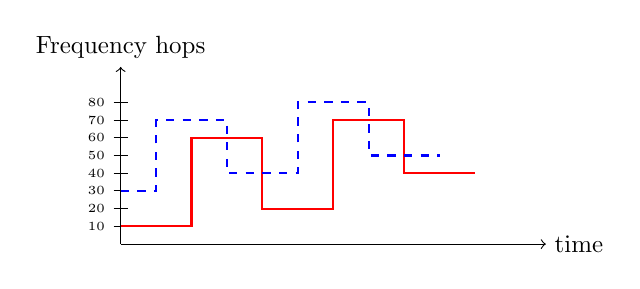
\begin{tikzpicture}[scale=0.9, transform shape]
            \draw[->] (0,0) -- (6,0) node[right] {time};
            \draw[->] (0,0) -- (0,2.5) node[above] {Frequency hops};
            \foreach \y in {10,20,...,80} {
                \draw (-0.1, \y/40) node[left] {\tiny \y} -- (0.1, \y/40);
            }
            \draw[thick, red] (0,10/40) -- (1,10/40) -- (1,60/40) -- (2,60/40) -- (2,20/40) -- (3,20/40) -- (3,70/40) -- (4,70/40) -- (4,40/40) -- (5,40/40);
            \draw[thick, blue, dashed] (0,30/40) -- (0.5,30/40) -- (0.5,70/40) -- (1.5,70/40) -- (1.5,40/40) -- (2.5,40/40) -- (2.5,80/40) -- (3.5,80/40) -- (3.5,50/40) -- (4.5,50/40);
        \end{tikzpicture}
        \caption{Esempio di Frequency Hopping Spread Spectrum (FHSS).}
        \label{fig:fhss}
        \end{figure}

        \item \textbf{Direct Sequence Spread Spectrum (DSSS):}
        \begin{itemize}
            \item Ogni bit di dati viene "espanso" moltiplicandolo per una sequenza di bit più lunga (detta "chipping code"). Questo distribuisce l'energia del segnale su una banda più larga.
            \item Per un ricevitore non sincronizzato, appare come rumore a larga banda di bassa potenza.
            \item \textit{Esempio:} Wi-Fi (802.11b) e GPS usano DSSS.
        \end{itemize}
         \begin{figure}[H]
        \centering
        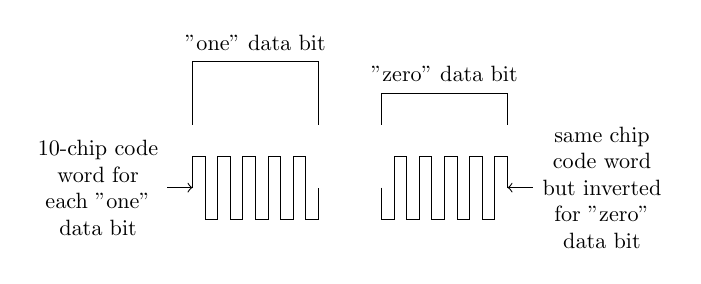
\begin{tikzpicture}[scale=0.8, transform shape]
            % "one" data bit
            \draw (0,1.5) -- (0,2.5) -- (2,2.5) -- (2,1.5);
            \node at (1,2.8) {"one" data bit};
            % 10-chip code for "one"
            \draw (0,0.5) -- (0,1) -- (0.2,1) -- (0.2,0) -- (0.4,0) -- (0.4,1) -- (0.6,1) -- (0.6,0) -- (0.8,0) -- (0.8,1) -- (1,1) -- (1,0) -- (1.2,0) -- (1.2,1) -- (1.4,1) -- (1.4,0) -- (1.6,0) -- (1.6,1) -- (1.8,1) -- (1.8,0) -- (2,0) -- (2,0.5);
            \node[text width=2cm, align=center] at (-1.5, 0.5) {10-chip code word for each "one" data bit};
            \draw[->] (-0.4,0.5) -- (0,0.5);

            % "zero" data bit
            \draw (3,1.5) -- (3,2) -- (5,2) -- (5,1.5);
            \node at (4,2.3) {"zero" data bit};
            % Inverted 10-chip code for "zero"
            \draw (3,0.5) -- (3,0) -- (3.2,0) -- (3.2,1) -- (3.4,1) -- (3.4,0) -- (3.6,0) -- (3.6,1) -- (3.8,1) -- (3.8,0) -- (4,0) -- (4,1) -- (4.2,1) -- (4.2,0) -- (4.4,0) -- (4.4,1) -- (4.6,1) -- (4.6,0) -- (4.8,0) -- (4.8,1) -- (5,1) -- (5,0.5);
            \node[text width=2cm, align=center] at (6.5, 0.5) {same chip code word but inverted for "zero" data bit};
            \draw[<-] (5,0.5) -- (5.4,0.5);
        \end{tikzpicture}
        \caption{Esempio di Direct Sequence Spread Spectrum (DSSS).}
        \label{fig:dsss_coding}
        \end{figure}
    \end{itemize}
    \item \textbf{Infrared Technology (Tecnologia Infrarossi):}
    \begin{itemize}
        \item Usa onde infrarosse. Richiede linea di vista o può essere diffusa in ambienti chiusi.
        \item \textit{Esempio:} Telecomandi TV.
    \end{itemize}
\end{itemize}

\section{Classificazione delle Reti Wireless per Copertura}
\begin{itemize}
    \item \textbf{WWAN (Wireless Wide Area Network):} Copertura geografica estesa (es. satelliti, reti cellulari).
    \item \textbf{WMAN (Wireless Metropolitan Area Network):} Copertura metropolitana (es. una città, WiMAX).
    \item \textbf{WLAN (Wireless Local Area Network):} Copertura locale (es. un edificio, una casa - Wi-Fi).
    \item \textbf{WPAN (Wireless Personal Area Network):} Copertura personale, ridotta (es. una stanza - Bluetooth).
    \item \textbf{Wireless Indoor Area Network:} Copertura a cortissimo raggio, tipicamente una stanza.
\end{itemize}
\textit{[Figura di riferimento: Slide 14 - Wireless network positioning]}

\section{Strutture delle Reti Wireless}
\subsection{WWAN e WMAN}
\begin{itemize}
    \item \textbf{Satelliti:}
    \begin{itemize}
        \item \textbf{LEO (Low Earth Orbit):} Orbita bassa.
        \item \textbf{GEO (Geostationary Orbit):} Orbita geostazionaria.
    \end{itemize}
    \textit{[Figura di riferimento: Slide 15 - Satelliti LEO e GEO]}
    \item \textbf{Reti Cellulari:} Evoluzione da 1G a 5G.
    \textit{[Figura di riferimento: Slide 16 - Wireless networks' structure (taxonomy)]}
    \item \textbf{Struttura Cellulare / Multi-Infrastructure WLAN:} Griglia di Access Points (AP) connessi a una Backbone.
    \textit{[Figura di riferimento: Slide 17 - Struttura multi-AP]}
\end{itemize}
\subsection{WLAN}
\begin{itemize}
    \item \textbf{Ad Hoc:}
    \begin{itemize}
        \item Comunicazione peer-to-peer (P2P) "al volo".
        \item Nessuna amministrazione centrale.
        \item \textit{Esempio:} Due laptop connessi direttamente via Wi-Fi.
    \end{itemize}
    \item \textbf{Infrastructure:}
    \begin{itemize}
        \item Unità di controllo centralizzata (Access Point).
        \item Roaming tra celle (AP).
        \item \textit{Esempio:} Tipica rete Wi-Fi domestica con router.
    \end{itemize}
\end{itemize}
\textit{[Figura di riferimento: Slide 18 - WLAN Ad Hoc vs Infrastructure]}

\section{Integrazione tra Mondo Wireless e Wired (Cablato)}
\begin{itemize}
    \item \textbf{Sfide:} Progettazione di protocolli wireless, integrazione, ottimizzazione (layering, bridging, Mobile IP, QoS).
    \item \textbf{Obiettivo:} Supportare applicazioni "wired-like" su dispositivi wireless.
    \item \textbf{Soluzione Possibile:}
    \begin{itemize}
        \item Scollegare reti wired e wireless per gestirle in modo indipendente ma interoperabile.
        \item Integrazione dei protocolli, mantenendo trasparenza.
        \item Strutture SW e protocolli per adattare contenuti a dispositivi eterogenei.
        \item Comportamento adattivo dei protocolli (lato wireless).
    \end{itemize}
\end{itemize}
\textit{[Figura di riferimento: Slide 19 - Wireless/Wired extension protocol stack]}

\section{Svantaggi (Drawbacks) del Wireless}
\begin{itemize}
    \item \textbf{Capacità di Canale Ridotta:} Inferiore alle reti cablate.
    \item \textbf{Spettro Limitato:} Risorsa scarsa. Necessità di riuso.
    \item \textbf{Energia Limitata (Batterie):} Sfida per dispositivi mobili.
    \item \textbf{Rumore e Interferenza:} Impatto elevato sulle prestazioni.
    \item \textbf{Sicurezza:} Informazioni "on the air", intercettabili.
    \item \textbf{Gestione della Mobilità:} Indirizzamento e routing (es. Mobile IP).
    \item \textbf{Tracciamento della Posizione (Location Tracking):} Paging, LBS.
    \item \textbf{Gestione della QoS (Quality of Service):} Complessa, multi-livello.
    \item \textbf{Servizi Best Effort:} Servizio base senza garanzie.
\end{itemize}

\section{Canale Logico Wireless e Multiplexing}
Il \textbf{multiplexing} permette a più utenti/segnali di condividere lo stesso mezzo trasmissivo.
\begin{itemize}
    \item \textbf{Dimensioni del Multiplexing:} Spazio ($s_i$), Tempo (t), Frequenza (f), Codice (c).
    \item \textbf{Importante:} Necessari "spazi di guardia" (guard spaces) per evitare interferenze.
\end{itemize}

\begin{figure}[H]
\centering
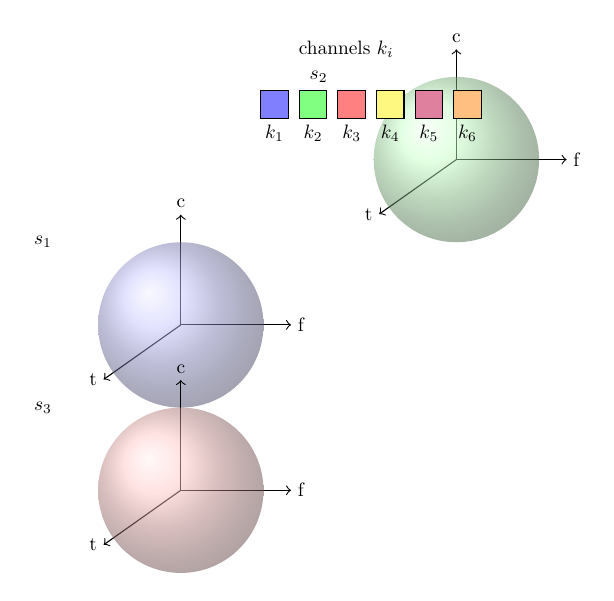
\begin{tikzpicture}[scale=0.7, transform shape]
    % Axes for s1
    \node at (-2.5,1.5) {$s_1$};
    \draw[->] (0,0) -- (2,0) node[right] {f};
    \draw[->] (0,0) -- (0,2) node[above] {c};
    \draw[->] (0,0) -- (-1.4,-1.4*0.707) node[left] {t}; % approx 45 deg projection
    \shade[ball color=blue!30, opacity=0.5] (0,0) circle (1.5cm);

    % Axes for s2 (shifted)
    \node at (2.5,1.5+3) {$s_2$};
    \draw[->] (5,0+3) -- (7,0+3) node[right] {f};
    \draw[->] (5,0+3) -- (5,2+3) node[above] {c};
    \draw[->] (5,0+3) -- (5-1.4,-1.4*0.707+3) node[left] {t};
    \shade[ball color=green!30, opacity=0.5] (5,3) circle (1.5cm);

    % Axes for s3 (shifted)
    \node at (-2.5,1.5-3) {$s_3$};
    \draw[->] (0,0-3) -- (2,0-3) node[right] {f};
    \draw[->] (0,0-3) -- (0,2-3) node[above] {c};
    \draw[->] (0,0-3) -- (-1.4,-1.4*0.707-3) node[left] {t};
    \shade[ball color=red!30, opacity=0.5] (0,-3) circle (1.5cm);

    % Channels k_i
    \node at (3, 5) {channels $k_i$};
    \foreach \i/\col in {1/blue,2/green,3/red,4/yellow,5/purple,6/orange}{
        \node[draw, fill=\col!50, minimum width=0.5cm, minimum height=0.5cm, label=below:$k_{\i}$] at (1+\i*0.7, 4) {};
    }
\end{tikzpicture}
\caption{Dimensioni del multiplexing (Spazio $s_i$, Tempo $t$, Frequenza $f$, Codice $c$).}
\label{fig:multiplex_dimensions}
\end{figure}

\subsection{Frequency Multiplex (FDM)}
\begin{itemize}
    \item L'intero spettro è diviso in bande di frequenza più piccole. Ogni canale ottiene una banda per tutto il tempo.
    \item \textbf{Vantaggi:} No coordinazione dinamica, funziona per segnali analogici.
    \item \textbf{Svantaggi:} Spreco di banda, inflessibile, spazi di guardia.
    \item \textit{Esempio:} Stazioni radio FM.
\end{itemize}
\begin{figure}[H]
\centering
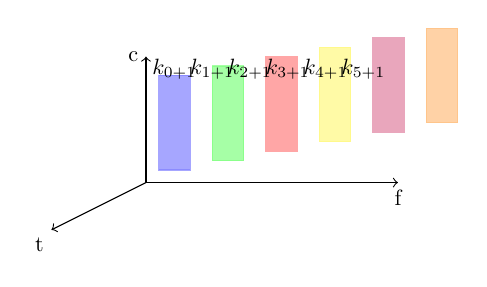
\begin{tikzpicture}[scale=0.8, transform shape,
    mychannel/.style={draw, minimum height=0.5cm, minimum width=3cm, opacity=0.7, transform shape}]
    \draw[->] (0,0) -- (0,2) node[left]{c};
    \draw[->] (0,0) -- (4,0) node[below]{f};
    \draw[->] (0,0) -- (-1.5,-0.75) node[below left]{t};
    \foreach \i/\col in {0/blue,1/green,2/red,3/yellow,4/purple,5/orange}{
      \fill[\col!50, mychannel,yshift=\i*0.5*0.3cm, xshift=\i*0.5*0.5cm] (0.2+\i*0.6,0.2) rectangle (0.2+\i*0.6+0.5, 0.2+1.5);
       \node at (0.45+\i*0.6, 1.8) {$k_{\i+1}$};
    }
\end{tikzpicture}
\caption{Frequency Division Multiplexing (FDM).}
\label{fig:fdm}
\end{figure}

\subsection{Time Multiplex (TDM)}
\begin{itemize}
    \item Un canale ottiene l'intero spettro per un certo periodo di tempo (time slot).
    \item \textbf{Vantaggi:} Solo un carrier alla volta, throughput elevato.
    \item \textbf{Svantaggi:} Precisa sincronizzazione necessaria.
    \item \textit{Esempio:} Slot di tempo in GSM.
\end{itemize}
\begin{figure}[H]
\centering
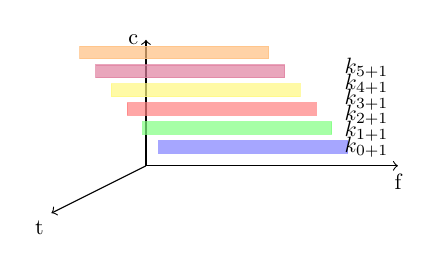
\begin{tikzpicture}[scale=0.8, transform shape,
    mychannel/.style={draw, minimum height=0.5cm, minimum width=0.5cm, opacity=0.7, transform shape}]
    \draw[->] (0,0) -- (0,2) node[left]{c};
    \draw[->] (0,0) -- (4,0) node[below]{f};
    \draw[->] (0,0) -- (-1.5,-0.75) node[below left]{t};
     \foreach \i/\col in {0/blue,1/green,2/red,3/yellow,4/purple,5/orange}{
      \fill[\col!50, mychannel, yshift=\i*0.05cm, xshift=-\i*0.25cm] (0.2, 0.2+\i*0.25) rectangle (0.2+3, 0.2+\i*0.25+0.2);
       \node at (3.5, 0.3+\i*0.25) {$k_{\i+1}$};
    }
\end{tikzpicture}
\caption{Time Division Multiplexing (TDM).}
\label{fig:tdm}
\end{figure}

\subsection{Time and Frequency Multiplex}
\begin{itemize}
    \item Combinazione: un canale ottiene una banda di frequenza per un periodo di tempo.
    \item \textit{Esempio:} GSM.
    \item \textbf{Vantaggi:} Migliore protezione, data rate più alti.
    \item \textbf{Svantaggi:} Precisa coordinazione.
\end{itemize}
\begin{figure}[H]
\centering
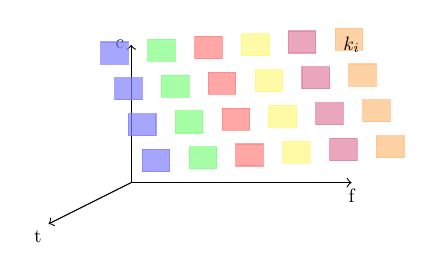
\begin{tikzpicture}[scale=0.7, transform shape,
    mychannel/.style={draw, minimum height=0.4cm, minimum width=0.5cm, opacity=0.7, transform shape}]
    \draw[->] (0,0) -- (0,2.5) node[left]{c};
    \draw[->] (0,0) -- (4,0) node[below]{f};
    \draw[->] (0,0) -- (-1.5,-0.75) node[below left]{t};
     \foreach \row in {0,...,3}{
        \foreach \colidx/\col in {0/blue,1/green,2/red,3/yellow,4/purple,5/orange}{
           \fill[\col!50, mychannel, yshift=\row*0.5*0.3cm + \colidx*0.5*0.1cm, xshift=-0.25*\row cm + \colidx*0.5*0.5cm]
            (0.2+\colidx*0.6, 0.2+\row*0.5) rectangle (0.2+\colidx*0.6+0.5, 0.2+\row*0.5+0.4);
        }
     }
     \node at (4,2.5) {$k_i$};
\end{tikzpicture}
\caption{Time and Frequency Multiplex.}
\label{fig:tdm_fdm}
\end{figure}

\subsection{Code Multiplex (CDM / CDMA)}
\begin{itemize}
    \item Ogni canale ha un codice univoco. Tutti usano lo stesso spettro nello stesso momento.
    \item \textbf{Vantaggi:} Efficienza di banda, no coordinazione stretta, buona protezione.
    \item \textbf{Svantaggi:} Data rate utente più bassi, rigenerazione complessa.
    \item Implementato con spread spectrum. \textit{Esempio:} Reti 3G.
\end{itemize}
\begin{figure}[H]
\centering
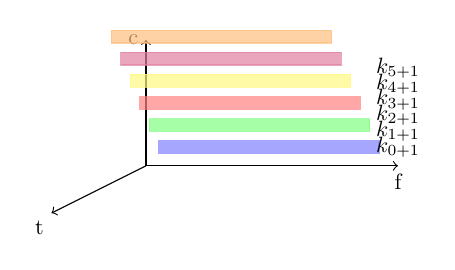
\begin{tikzpicture}[scale=0.8, transform shape,
    mychannel/.style={draw, minimum height=0.2cm, opacity=0.7, transform shape}]
    \draw[->] (0,0) -- (0,2) node[left]{c};
    \draw[->] (0,0) -- (4,0) node[below]{f};
    \draw[->] (0,0) -- (-1.5,-0.75) node[below left]{t};
     \foreach \i/\col in {0/blue,1/green,2/red,3/yellow,4/purple,5/orange}{
      \fill[\col!50, mychannel, yshift=\i*0.1cm, xshift=-\i*0.15cm] (0.2, 0.2+\i*0.25) rectangle (0.2+3.5, 0.2+\i*0.25+0.2);
      \node at (4, 0.3+\i*0.25) {$k_{\i+1}$};
    }
\end{tikzpicture}
\caption{Code Division Multiplexing (CDM).}
\label{fig:cdm}
\end{figure}

\section{Pianificazione delle Frequenze}
\begin{itemize}
    \item \textbf{Riuso delle Frequenze:} Le stesse frequenze possono essere riutilizzate in celle non adiacenti.
    \item \textbf{Modello Standard a 7 Frequenze:} Pattern comune per allocare frequenze.
    \item \textbf{Assegnazione Fissa vs. Dinamica.}
\end{itemize}
\begin{figure}[H]
\centering
\begin{tikzpicture}[scale=0.8, transform shape,
    hexagon/.style={regular polygon, regular polygon sides=6, minimum size=1.5cm, draw, thick}]
    \node[hexagon, label=center:$f_1$] (c1) {};
    \node[hexagon, label=center:$f_2$, right=0.01cm of c1, anchor=west, xshift=-0.38cm, yshift=0.65cm] (c2) {};
    \node[hexagon, label=center:$f_3$, right=0.01cm of c2, anchor=west, xshift=-0.38cm, yshift=0.65cm] (c3) {};
    \node[hexagon, label=center:$f_4$, right=0.01cm of c1, anchor=west, xshift=-0.38cm, yshift=-0.65cm] (c4) {};
    \node[hexagon, label=center:$f_5$, right=0.01cm of c4, anchor=west, xshift=-0.38cm, yshift=-0.65cm] (c5) {};
    \node[hexagon, label=center:$f_6$, left=0.01cm of c1, anchor=east, xshift=0.38cm, yshift=0.65cm] (c6) {};
    \node[hexagon, label=center:$f_7$, left=0.01cm of c1, anchor=east, xshift=0.38cm, yshift=-0.65cm] (c7) {};
\end{tikzpicture}
\caption{Cluster di 7 celle per il riuso delle frequenze.}
\label{fig:frequency_planning}
\end{figure}

\section{Modulazione}
Processo di variare proprietà di un segnale portante con un segnale modulante.
\begin{itemize}
    \item \textbf{Modulazione Digitale:} Dati digitali $\rightarrow$ segnale analogico (baseband).
    \begin{itemize}
        \item \textbf{ASK (Amplitude Shift Keying)}
        \item \textbf{FSK (Frequency Shift Keying)}
        \item \textbf{PSK (Phase Shift Keying)}
    \end{itemize}
    \item \textbf{Modulazione Analogica (su portante RF):} Sposta il segnale baseband sulla portante radio.
    \item \textbf{Motivazione:} Antenne più piccole, FDM, caratteristiche del mezzo.
    \item \textbf{Schemi Base (per portante RF):} AM, FM, PM.
\end{itemize}

\subsection{Processo di Trasmissione di Bit con Onde Radio}
\begin{figure}[H]
\centering
\begin{tikzpicture}[node distance=1.5cm, auto,
    block/.style={rectangle, draw, fill=blue!20, text width=7em, text centered, rounded corners, minimum height=2em},
    line/.style={draw, -latex},
    wave/.style={draw, -latex, decorate, decoration={snake}}]

    \node [text width=6em] (info_in) {Info Digitale 101101001};
    \node [block, right=of info_in] (dig_mod) {Modulazione Digitale};
    \node [block, right=2.5cm of dig_mod] (ana_mod) {Modulazione Analogica};
    \node [text width=6em, right=of ana_mod] (radio_out) {Emissione Radio (segnale RF)};
    \node [coordinate, below=0.5cm of dig_mod] (baseband_mid) {};
    \node [coordinate, below=0.5cm of ana_mod] (carrier_mid) {};

    \draw [line] (info_in) -- (dig_mod);
    \draw [line, dashed] (dig_mod.east) -- node[midway,above,yshift=0.1cm] {\tiny Analog (baseband)} (ana_mod.west);
    \draw [line, dashed] (ana_mod.south) ++(0,-0.1) -- node[midway,right,xshift=0.1cm] {\tiny Carrier} (carrier_mid);
    \draw [line, dashed] (ana_mod.east) -- (radio_out.west);

    % Ricezione
    \node [text width=6em, below=3cm of radio_out] (radio_in) {Segnale RF ricevuto};
    \node [block, left=of radio_in] (ana_demod) {Demod. Analogica};
    \node [block, left=2.5cm of ana_demod] (dig_demod) {Interpret. (Demod. Digit.)};
    \node [text width=6em, left=of dig_demod] (info_out) {Info Digitale (es. 101111000)};
    \node [coordinate, below=0.5cm of ana_demod] (carrier_mid_rx) {};
    \node [coordinate, below=0.5cm of dig_demod] (baseband_mid_rx) {};

    \draw [line] (radio_in.west) -- (ana_demod.east);
    \draw [line, dashed] (ana_demod.south) ++(0,-0.1) -- node[midway,right,xshift=0.1cm] {\tiny Carrier} (carrier_mid_rx);
    \draw [line, dashed] (ana_demod.west) -- node[midway,above,yshift=0.1cm] {\tiny Analog (baseband)} (dig_demod.east);
    \draw [line] (dig_demod.west) -- (info_out.east);

    % Canale con problemi
    \path (radio_out.south) edge[line, bend right=20, dashed, red] node[midway, below, yshift=-0.2cm, text width=5em] {Canale (Rumore, Interferenze)} (radio_in.north);

\end{tikzpicture}
\caption{Processo di modulazione e demodulazione.}
\label{fig:mod_demod_process}
\end{figure}
\textit{L'analogia del test di Ishihara (Slide 34-35) illustra l'effetto del rumore: un segnale chiaro è facile da interpretare, uno rumoroso no.}

\section{Tecniche di Modulazione Digitale (Shift Keying)}
\begin{figure}[H]
\centering
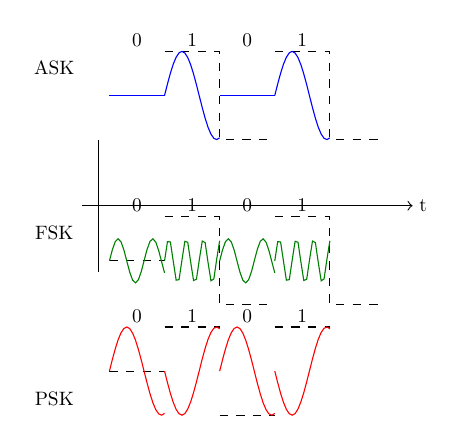
\begin{tikzpicture}[scale=0.7, transform shape]
    \draw[->] (-0.5,0) -- (5.5,0) node[right]{t};
    \draw (-0.2,-1.2) -- (-0.2,1.2);
    % ASK
    \node at (-1, 2.5) {ASK};
    \draw[dashed] (0,2) -- (1,2) (1,2.8) -- (2,2.8) -- (2,1.2) -- (3,1.2) (3,2.8) -- (4,2.8) -- (4,1.2) -- (5,1.2); % Bits 0 1 0 1
    \draw[blue, domain=1:2, samples=20, variable=\x] plot (\x, {0.8*sin(5*(\x-1) r) + 2}); % 1
    \draw[blue] (0,2) -- (1,2); % 0
    \draw[blue, domain=3:4, samples=20, variable=\x] plot (\x, {0.8*sin(5*(\x-3) r) + 2}); % 1
    \draw[blue] (2,2) -- (3,2); % 0
    \node at (0.5,3) {0}; \node at (1.5,3) {1}; \node at (2.5,3) {0}; \node at (3.5,3) {1};

    % FSK
    \node at (-1, -0.5) {FSK};
    \draw[dashed] (0,-1) -- (1,-1) (1, -0.2) -- (2,-0.2) -- (2,-1.8) -- (3,-1.8) (3,-0.2) -- (4,-0.2) -- (4,-1.8) -- (5,-1.8);
    \draw[green!50!black, domain=0:1, samples=20, variable=\x] plot (\x, {0.4*sin(10*\x r) -1}); % Low freq for 0
    \draw[green!50!black, domain=1:2, samples=20, variable=\x] plot (\x, {0.4*sin(20*(\x-1) r) -1}); % High freq for 1
    \draw[green!50!black, domain=2:3, samples=20, variable=\x] plot (\x, {0.4*sin(10*(\x-2) r) -1}); % Low freq for 0
    \draw[green!50!black, domain=3:4, samples=20, variable=\x] plot (\x, {0.4*sin(20*(\x-3) r) -1}); % High freq for 1
    \node at (0.5,0) {0}; \node at (1.5,0) {1}; \node at (2.5,0) {0}; \node at (3.5,0) {1};

    % PSK
    \node at (-1, -3.5) {PSK};
    \draw[dashed] (0,-3) -- (1,-3) (1,-2.2) -- (2,-2.2) (2,-3.8) -- (3,-3.8) (3,-2.2) -- (4,-2.2);
    \draw[red, domain=0:1, samples=20, variable=\x] plot (\x, {0.8*sin(5*\x r) -3}); % Phase 0 for 0
    \draw[red, domain=1:2, samples=20, variable=\x] plot (\x, {0.8*sin(5*(\x-1) r + pi r) -3}); % Phase pi for 1
    \draw[red, domain=2:3, samples=20, variable=\x] plot (\x, {0.8*sin(5*(\x-2) r) -3}); % Phase 0 for 0
    \draw[red, domain=3:4, samples=20, variable=\x] plot (\x, {0.8*sin(5*(\x-3) r + pi r) -3}); % Phase pi for 1
    \node at (0.5,-2) {0}; \node at (1.5,-2) {1}; \node at (2.5,-2) {0}; \node at (3.5,-2) {1};
\end{tikzpicture}
\caption{Tecniche di Shift Keying: ASK, FSK, PSK.}
\label{fig:shift_keying}
\end{figure}
\begin{itemize}
    \item \textbf{ASK:} Semplice (ON/OFF), poche risorse di spettro, suscettibile a interferenze.
    \item \textbf{FSK:} Usa più spettro, due frequenze per '1' e '0', più robusta di ASK.
    \item \textbf{PSK:} Più complessa, più robusta, varia la fase della portante.
\end{itemize}

\section{Rappresentazione del Segnale}
\begin{itemize}
    \item \textbf{Dominio dell'Ampiezza:} Amiezza (V) vs Tempo (s).
    \item \textbf{Dominio della Frequenza:} Ampiezza vs Frequenza (Hz).
    \item \textbf{Diagramma di Fase e Ampiezza (Diagramma di Costellazione / IQ):}
    Rappresenta ampiezza (M) e fase ($\phi$) in coordinate polari. Asse I (In-phase): $M \cos \phi$, Asse Q (Quadrature): $M \sin \phi$. Ogni \textbf{SIMBOLO} è un punto.
\end{itemize}
\begin{figure}[H]
\centering
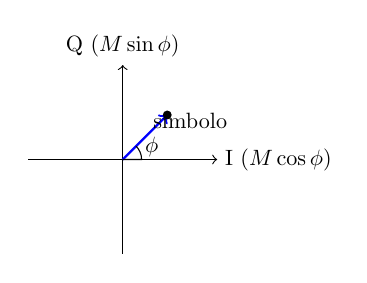
\begin{tikzpicture}[scale=0.8, transform shape]
    \draw[->] (-1.5,0) -- (1.5,0) node[right] {I ($M \cos \phi$)};
    \draw[->] (0,-1.5) -- (0,1.5) node[above] {Q ($M \sin \phi$)};
    \coordinate (O) at (0,0);
    \coordinate (P) at (45:1); % Esempio: M=1, phi=45 deg
    \draw[thick, blue, ->] (O) -- (P) node[midway, above right, black] {simbolo};
    \draw (O) -- (0.3,0) arc (0:45:0.3);
    \node at (22.5:0.5) {$\phi$};
    \fill (P) circle (2pt);
\end{tikzpicture}
\caption{Diagramma di Costellazione (IQ).}
\label{fig:iq_diagram}
\end{figure}

\section{Esempi di Modulazione PSK e QAM}
\subsection{BPSK (Binary Phase Shift Keying)}
\begin{itemize}
    \item Ogni simbolo = 1 bit. Bit 0: fase 0°; Bit 1: fase 180°.
    \item Semplice, robusta. Bassa efficienza spettrale.
\end{itemize}
\begin{figure}[H] \centering
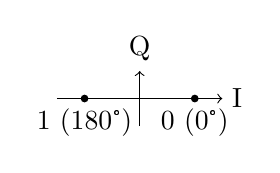
\begin{tikzpicture}[scale=0.7]
    \draw[->] (-1.5,0) -- (1.5,0) node[right] {I}; \draw[->] (0,-0.5) -- (0,0.5) node[above] {Q};
    \fill (1,0) circle (2pt) node[below] {0 (0°)}; \fill (-1,0) circle (2pt) node[below] {1 (180°)};
\end{tikzpicture} \caption{BPSK IQ Diagram.} \end{figure}

\subsection{QPSK (Quadrature Phase Shift Keying)}
\begin{itemize}
    \item Ogni simbolo = 2 bit (es. 00: +45°, 01: +135°, 10: +225°, 11: +315°).
    \item Più complessa e vulnerabile, ma doppia efficienza spettrale.
\end{itemize}
\begin{figure}[H] \centering
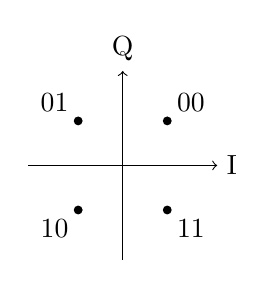
\begin{tikzpicture}[scale=0.8]
    \draw[->] (-1.5,0) -- (1.5,0) node[right] {I}; \draw[->] (0,-1.5) -- (0,1.5) node[above] {Q};
    \fill (0.707,0.707) circle (2pt) node[above right] {00}; % 45
    \fill (-0.707,0.707) circle (2pt) node[above left] {01};  % 135
    \fill (-0.707,-0.707) circle (2pt) node[below left] {10}; % 225
    \fill (0.707,-0.707) circle (2pt) node[below right] {11}; % 315
\end{tikzpicture} \caption{QPSK IQ Diagram.} \end{figure}

\subsection{Analogia "Tiro al Bersaglio" e Area del Bersaglio}
\begin{itemize}
    \item Il trasmettitore "lancia" simboli. Il ricevitore interpreta il simbolo "più vicino".
    \item \textbf{Canale Rumoroso:} Si usa BPSK (bersagli grandi/lontani).
    \item \textbf{Canale Buono:} Si usa QPSK/QAM (più bit/simbolo, bersagli più piccoli/vicini).
\end{itemize}

\subsection{Associazione Bit-Simboli (Gray Coding)}
\begin{itemize}
    \item \textbf{Gray Coding:} Simboli adiacenti nel diagramma IQ differiscono per un solo bit.
    \item Minimizza gli errori di bit: se un simbolo è confuso con uno adiacente, solo 1 bit è errato.
\end{itemize}
\begin{figure}[H] \centering
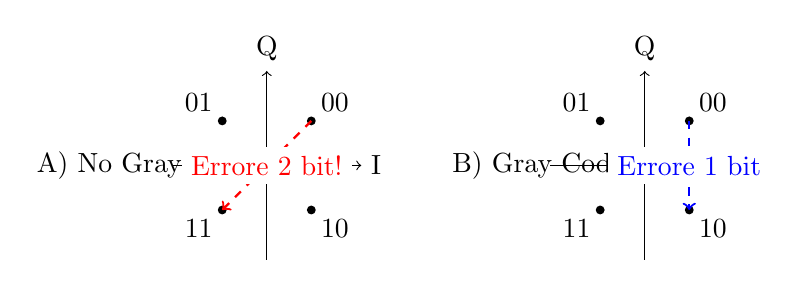
\begin{tikzpicture}[scale=0.8]
    \node at (-2.5,0) {A) No Gray};
    \draw[->] (-1.5,0) -- (1.5,0) node[right] {I}; \draw[->] (0,-1.5) -- (0,1.5) node[above] {Q};
    \fill (0.707,0.707) circle (2pt) node[above right] {00};
    \fill (-0.707,0.707) circle (2pt) node[above left] {01};
    \fill (-0.707,-0.707) circle (2pt) node[below left] {11}; % Errore di 2 bit se da 00
    \fill (0.707,-0.707) circle (2pt) node[below right] {10};
    \draw[red, thick, dashed, ->] (0.707,0.707) -- (-0.707,-0.707) node[midway, fill=white, text=red] {Errore 2 bit!};

    \node at (4.5,0) {B) Gray Coding};
    \begin{scope}[xshift=6cm]
    \draw[->] (-1.5,0) -- (1.5,0) node[right] {I}; \draw[->] (0,-1.5) -- (0,1.5) node[above] {Q};
    \fill (0.707,0.707) circle (2pt) node[above right] {00};
    \fill (-0.707,0.707) circle (2pt) node[above left] {01};
    \fill (-0.707,-0.707) circle (2pt) node[below left] {11}; % Gray coded
    \fill (0.707,-0.707) circle (2pt) node[below right] {10}; % Gray coded
    \draw[blue, thick, dashed, ->] (0.707,0.707) -- (0.707,-0.707) node[midway, fill=white, text=blue] {Errore 1 bit};
    \end{scope}
\end{tikzpicture} \caption{Confronto Gray Coding (NB: etichette simboli semplificate).} \end{figure}

\subsection{Rilevamento e Correzione Errori}
\begin{itemize}
    \item \textbf{Bit di Parità:} Rileva errori singoli.
    \item \textbf{Matrice di Bit di Parità:} Permette di identificare e correggere un singolo bit errato.
\end{itemize}

\subsection{QAM (Quadrature Amplitude Modulation)}
\begin{itemize}
    \item Combina modulazione di ampiezza E di fase. $2^n$ simboli, $n$ bit/simbolo.
    \item \textbf{16-QAM:} 16 simboli, 4 bit/simbolo.
    \item Area del "bersaglio" si riduce con $n$, più sensibile al rumore ma più efficiente.
\end{itemize}
\begin{figure}[H] \centering
\begin{tikzpicture}[scale=0.7]
    \draw[->] (-2.5,0) -- (2.5,0) node[right] {I}; \draw[->] (0,-2.5) -- (0,2.5) node[above] {Q};
    \foreach \x in {-1.5, -0.5, 0.5, 1.5} {
        \foreach \y in {-1.5, -0.5, 0.5, 1.5} {
            \fill (\x,\y) circle (2pt);
        }
    }
    \node at (0.5,0.5) [above right, font=\tiny, red] {0000}; % Esempio
    \node at (1.5,0.5) [above right, font=\tiny, red] {0001}; % Esempio
    \node at (0.5,1.5) [above right, font=\tiny, red] {0010}; % Esempio
\end{tikzpicture} \caption{16-QAM IQ Diagram (16 simboli).} \end{figure}

\subsection{Modulazione Gerarchica}
\begin{itemize}
    \item Modula due sequenze di bit con priorità diverse.
    \item \textbf{Esempio 64-QAM Gerarchica (Videochiamata):}
    \begin{itemize}
        \item 6 bit/simbolo. Diagramma IQ diviso in 4 "gray clouds" (quadranti).
        \item 4 bit (bassa priorità, video) per i sotto-simboli nella cloud.
        \item 2 bit (alta priorità, voce) per etichettare la cloud.
        \item \textbf{Basso Rumore:} Voce e video OK.
        \item \textbf{Alto Rumore:} Errori video, ma voce preservata (cloud corretta identificata).
    \end{itemize}
\end{itemize}
\textit{[Figura di riferimento: Slide 61-77 - Hierarchical Modulation]}

\section{Tecniche Avanzate di Trasmissione e Accesso Multiplo}
\subsection{Spreading e Fading Selettivo in Frequenza}
\textit{[Figura di riferimento: Slide 79 - Spreading and frequency selective fading]}
\begin{itemize}
    \item Il \textit{fading} è un'attenuazione del segnale dipendente dalla frequenza.
    \item Lo \textit{spread spectrum} distribuisce l'energia su una banda più ampia, rendendo il segnale più robusto.
\end{itemize}

\subsection{DSSS (Direct Sequence Spread Spectrum) - Dettagli}
\textit{[Figure di riferimento: Slide 80-83 - DSSS I, II]}
\begin{itemize}
    \item XOR del segnale dati con una \textit{chipping sequence}.
    \item Molti "chip" per bit $\rightarrow$ maggiore larghezza di banda.
    \item \textbf{Assegnazione Canali IEEE 802.11b (DSSS):} Canali non sovrapposti (es. 1, 6, 11) per evitare interferenze.
\end{itemize}
\begin{figure}[H]
\centering
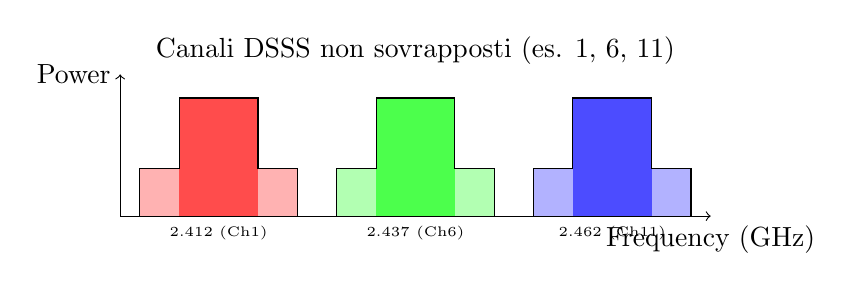
\begin{tikzpicture}[yscale=0.6,xscale=0.5]
    \draw[->] (0,0) -- (15,0) node[below] {Frequency (GHz)};
    \draw[->] (0,0) -- (0,3) node[left] {Power};
    \node[below, font=\tiny] at (2.5,0) {2.412 (Ch1)};
    \node[below, font=\tiny] at (7.5,0) {2.437 (Ch6)};
    \node[below, font=\tiny] at (12.5,0) {2.462 (Ch11)};
    \foreach \center/\col in {2.5/red, 7.5/green, 12.5/blue}{
        \fill[\col!30] (\center-2,0) rectangle (\center+2,1); % Sidelobes
        \fill[\col!70] (\center-1,0) rectangle (\center+1,2.5); % Mainlobe
        \draw (\center-2,0) -- (\center-2,1) -- (\center-1,1) -- (\center-1,2.5) -- (\center+1,2.5) -- (\center+1,1) -- (\center+2,1) -- (\center+2,0);
    }
    \node at (7.5, 3.5) {Canali DSSS non sovrapposti (es. 1, 6, 11)};
\end{tikzpicture}
\caption{Esempio di canali DSSS non sovrapposti in IEEE 802.11b.}
\label{fig:dsss_channels}
\end{figure}

\subsection{CDMA (Code Division Multiple Access) - Dettagli}
\textit{[Figure di riferimento: Slide 86-91 - CDMA]}
\begin{itemize}
    \item Usa DSSS. Ogni utente ha un codice univoco.
    \item Tutti trasmettono sulla stessa frequenza contemporaneamente.
    \item Il ricevitore usa il codice per estrarre il segnale desiderato.
\end{itemize}

\subsection{FHSS (Frequency Hopping Spread Spectrum) - Dettagli}
\textit{[Figure di riferimento: Slide 92-94 - FHSS I, II, III]}
\begin{itemize}
    \item Cambiamenti discreti della frequenza portante.
    \item \textbf{Fast Hopping:} Diverse frequenze/bit. \textbf{Slow Hopping:} Diversi bit/frequenza.
\end{itemize}

\subsection{OFDM (Orthogonal Frequency Division Multiplexing)}
\textit{[Figure di riferimento: Slide 95-100 - OFDM]}
\begin{itemize}
    \item Trasmette dati su molte \textbf{sottoportanti (subcarriers)} parallele ortogonali.
    \item \textbf{Vantaggi:} Alta efficienza spettrale, robustezza al multipath fading.
    \item \textbf{Funzionamento (semplificato):} Flusso bit diviso $\rightarrow$ ogni parte modula una sottoportante $\rightarrow$ IFFT per creare segnale tempo $\rightarrow$ trasmissione $\rightarrow$ FFT al ricevitore per separare.
    \item Usato in Wi-Fi (802.11a/g/n/ac/ax), WiMAX, LTE/5G, DVB-T.
\end{itemize}
\begin{table}[H]
\centering
\caption{Esempio Riassuntivo OFDM (IEEE 802.11a/g - valori indicativi)}
\label{tab:ofdm_summary}
\begin{tabular}{|c|c|c|c|c|c|}
\hline
\textbf{Data Rate} & \textbf{Modulazione} & \textbf{Bit/simbolo} & \textbf{Coding Rate} & \textbf{Bit Dati} & \textbf{Bit Utili} \\
\textbf{(Mbps)} & \textbf{(per subcarrier)} & \textbf{(per subcarrier)} & \textbf{R (dati/tot)} & \textbf{per simbolo OFDM} & \textbf{per simbolo OFDM}\\
\hline
6  & BPSK  & 1 & 1/2 & $48 \times 1 = 48$  & $48 \times 1/2 = 24$ \\
9  & BPSK  & 1 & 3/4 & $48 \times 1 = 48$  & $48 \times 3/4 = 36$ \\
12 & QPSK  & 2 & 1/2 & $48 \times 2 = 96$  & $96 \times 1/2 = 48$ \\
18 & QPSK  & 2 & 3/4 & $48 \times 2 = 96$  & $96 \times 3/4 = 72$ \\
24 & 16-QAM & 4 & 1/2 & $48 \times 4 = 192$ & $192 \times 1/2 = 96$ \\
36 & 16-QAM & 4 & 3/4 & $48 \times 4 = 192$ & $192 \times 3/4 = 144$ \\
48 & 64-QAM & 6 & 2/3 & $48 \times 6 = 288$ & $288 \times 2/3 = 192$ \\
54 & 64-QAM & 6 & 3/4 & $48 \times 6 = 288$ & $288 \times 3/4 = 216$ \\
\hline
\multicolumn{6}{l}{\footnotesize Basato su 48 data subcarriers, simbolo OFDM di $4\mu s$. Bit Dati = Subcarriers * Bit/simbolo.} \\
\multicolumn{6}{l}{\footnotesize Bit Utili = Bit Dati * Coding Rate.} \\
\end{tabular}
\end{table}


\section{Conclusione Generale}
La differenza tra trasmissioni wireless "buone" e "cattive", a parità di condizioni fisiche, risiede principalmente nelle \textbf{scelte intelligenti} riguardanti:
\begin{itemize}
    \item Componenti di protocollo efficienti ed efficaci.
    \item Strutture dati e algoritmi.
    \item Avanzamenti hardware.
\end{itemize}
Il tutto utilizzato in modo da basarsi su assunzioni corrette e sfruttare al meglio le opportunità per trasformare svantaggi o limiti in vantaggi pratici o sinergie. Gli esempi chiariscono il ruolo attivo e rilevante dei \textbf{protocolli} nel raggiungere il potenziale di trasmissione in un mondo "ostile".

\end{document}